\documentclass{sigchi}

% Use this command to override the default ACM copyright statement (e.g. for preprints). 
% Consult the conference website for the camera-ready copyright statement.


% Arabic page numbers for submission. 
% Remove this line to eliminate page numbers for the camera ready copy
%\pagenumbering{arabic}



\usepackage{balance}  % to better equalize the last page
\usepackage{graphics} % for EPS, load graphicx instead
\usepackage{times}    % comment if you want LaTeX's default font
\usepackage{url}      % llt: nicely formatted URLs
\usepackage{graphicx}
\usepackage{caption}
\usepackage{subcaption}
\usepackage{array}
%\usepackage{multirow}

% llt: Define a global style for URLs, rather that the default one
\makeatletter
\def\url@leostyle{%
  \@ifundefined{selectfont}{\def\UrlFont{\sf}}{\def\UrlFont{\small\bf\ttfamily}}}
\makeatother
\urlstyle{leo}


% To make various LaTeX processors do the right thing with page size.
\def\pprw{8.5in}
\def\pprh{11in}
\special{papersize=\pprw,\pprh}
\setlength{\paperwidth}{\pprw}
\setlength{\paperheight}{\pprh}
\setlength{\pdfpagewidth}{\pprw}
\setlength{\pdfpageheight}{\pprh}

% Make sure hyperref comes last of your loaded packages, 
% to give it a fighting chance of not being over-written, 
% since its job is to redefine many LaTeX commands.
%\usepackage[pdftex]{hyperref}
%\hypersetup{
%pdftitle={L@S 2014 Work-in-Progress Format},
%pdfauthor={LaTeX},
%pdfkeywords={SIGCHI, proceedings, archival format},
%bookmarksnumbered,
%pdfstartview={FitH},
%colorlinks,
%citecolor=black,
%filecolor=black,
%linkcolor=black,
%urlcolor=black,
%breaklinks=true,
%}

% create a shortcut to typeset table headings
\newcommand\tabhead[1]{\small\textbf{#1}}

\begin{document}

\title{Making the Grade}
\large

\numberofauthors{2}
\author{
  \alignauthor Casey O'Brien\\
    \email{cmobrien@mit.edu}
\alignauthor Adam Yedidia\\
\email{adamy@mit.edu}
}

\maketitle

\section{Abstract}

\section{Introduction}

Say that you are a student in a large introductory class, like 6.006. Halfway through the semester, you'd really like to know: \textit{How likely is it that I get an A in this class?}

As TA�s for 6.006, we field questions like this all the time. We answer them with a very practiced response, something like: \textit{We cannot make any predictions about final grades before all assignments are graded}. We say this because we do not want to risk making an incorrect prediction and having the student complain at the end of the semester. However, this is basically a blatant lie. In fact, we think that given a student's grades halfway through the semester, we can make a fairly accurate prediction as to what their final grade in the course will be.

Our work will focus on 6.006, \textit{Introduction to Algorithms}. For the past five years, very little about the class has changed. Each semester, there are 9 assignments: 6 problem sets, 2 quizzes, and a final exam. A student's final numerical grade is weighted as 5\% per problem set, 20\% per quiz, and 30\% for the final exam.

There are three different types of problem that we will discuss in this paper.
\begin{enumerate}
\item \textit{Numerical Prediction}: Predict the student's final numerical average.
\item \textit{Letter Prediction}: Predict the student's final letter grade.
\item \textit{Letter Distribution}: Find the probability distribution over a student's final letter grade.
\end{enumerate}

We solved all of these problems at each point throughout the class (i.e., after each assignment was due). This allowed us to see how our predictive power increased as we progressed throughout the semester. As one might expect, we saw the largest decreases in our error rates after each of the quizzes.

To compute the numerical prediction, we used regression. For letter prediction, we tried two different models. The first was to perform regression, and then map numerical scores to letter grades. The second was to use an ordered logit/probit model, which, in turn, solved the letter distribution problem. These models will be discussed in more detail in the coming sections.

\subsection{Data}

We have grade data for six semesters over the past five years. For each student, we have their grade on each assignment, as well as their final letter grade in the class. Within any semester, professors used hard thresholds for letter grade divides. So, if Alice and Bob took 6.006 in the same semester, and Alice has a higher weighted average than Bob, then Alice's letter grade is at least as good as Bob's.

Figure 1 displays information about our dataset. In particular, Figure 1(a) shows the distribution of students over the different majors (note that double majors were counted in both corresponding columns). We can see that almost all students are either courses 6 or 18. Figure 1(b) shows the gender distribution (which is about 2:1 male:female). Figure 1(c) shows the year distribution, where we see that the students are mostly sophomores. Finally, Figure 1(d) shows the distribution over final grades, which is about 41\% A's, 41\% B's, and 18\% C's. Note that this distribution varies slightly across different semesters.

\begin{figure*}[t!]

\begin{tabular}{c c c}
\multicolumn{3}{ c }{
	\begin{subfigure}[b]{7in}
		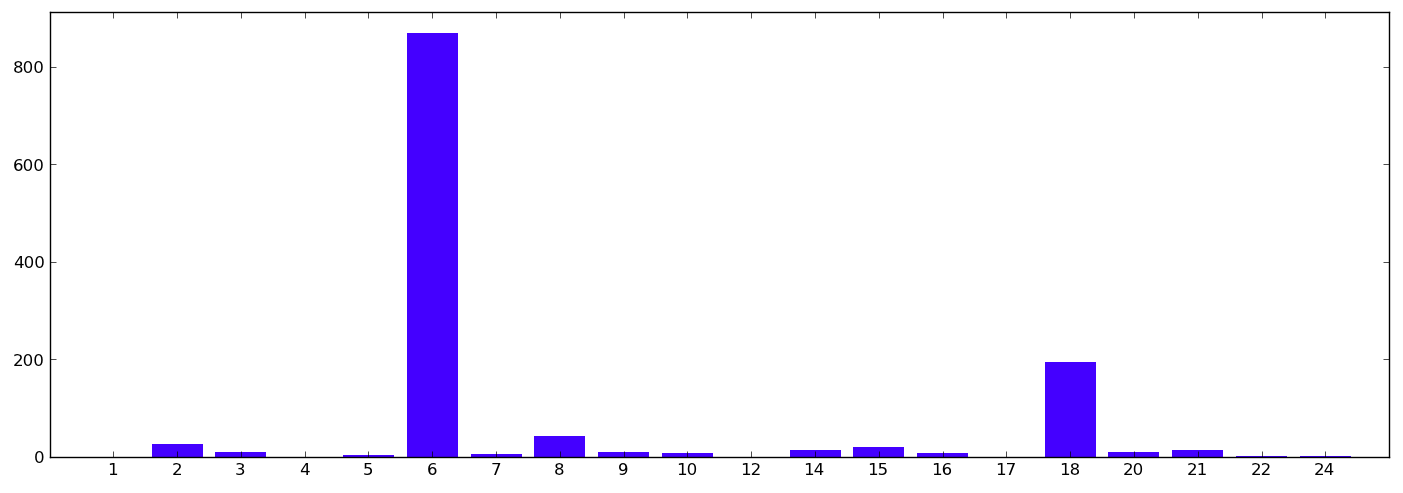
\includegraphics[width=7in]{plots/major.png}
		\caption{CAPTION}
	\end{subfigure}
	}
\\ &&\\
\begin{subfigure}[b]{2.25in}
	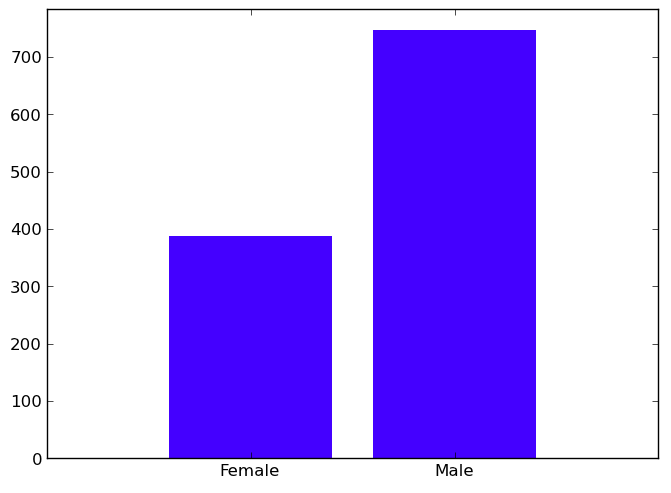
\includegraphics[width=2.25in]{plots/gender.png}
	\caption{CAPTION}
\end{subfigure}
&
\begin{subfigure}[b]{2.25in}
	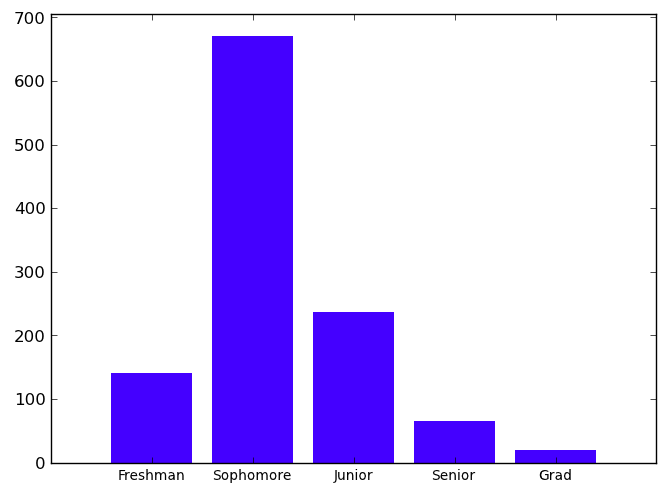
\includegraphics[width=2.25in]{plots/year.png}
	\caption{CAPTION}
\end{subfigure}
&
\begin{subfigure}[b]{2.25in}
	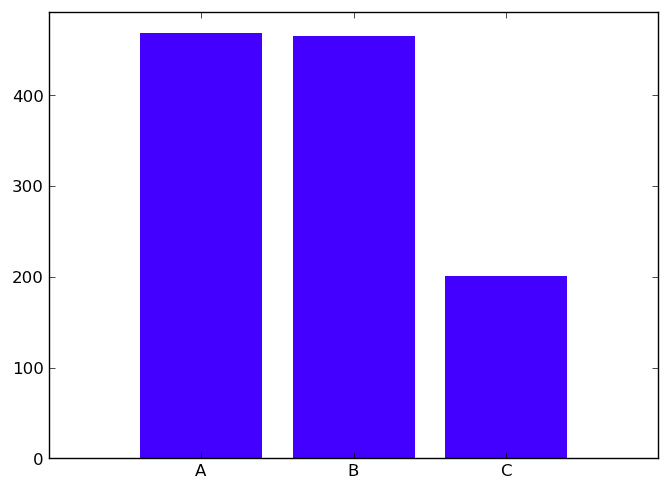
\includegraphics[width=2.25in]{plots/grade.png}
	\caption{CAPTION}
\end{subfigure}
\end{tabular}

\caption{Caption}

\end{figure*}

We would like for our models to be able to predict scores not just in these six semesters, but in future semesters. When this is being used in the future, the test data will consist of students from a single semester, and the goal will be to predict their final grades before we actually know them. As such, we randomly chose a single semester of the six to represent our test data. The test data consists of 197 students. The other five semesters, consisting of 938 students in total, were combined and used as training and validation data.

\subsection{Features}

The first, most obvious features to include were the assignment grades. For each assignment (of the assignments being considered at the time), we included as a feature the difference between the student's score and the mean.  We considered dividing by the standard deviation of the assignment (to get the $z$-score), but we realized this has a key flaw. The weighted sum of the $z$-scores of assignments is not equal to the $z$-score of the weighted sum of raw scores. The result is that when students are sorted by weighted sum of $z$-scores, we no longer have the property that grades obey hard thresholds, as described above.

This is perhaps an interesting issue to consider about the way that we assign grades. Say that Alice scores 20 points below average on a test with a very high variance and 20 points above average on a test with very low variance. Bob, on the other hand, scores 20 points above average on the high variance test and 20 points below average on the low variance test. It seems clear that Alice is performing better in the class, yet by our current grading scheme, both students have the same overall score.

Of course, since all of the semesters for which we have data were not graded using $z$-scores, we do not consider this idea any further here.

In order to make it easier to comprehend the weights resulting from our models, we scaled problem set features to be out of 5 (before subtracting the mean), quiz features out of 20, and the final feature out of 30. The result is that when we compare the weights for say, a problem set and a quiz, we can directly compare the effects of a 1\% change to final score caused by a problem set and a 1\% change to final score caused by a quiz.

Another feature we included is the number of zeros scored on problem sets. For various reasons, some students do not complete certain problem sets throughout the semester. If we are told that a student has an average of 50\% on problem sets after the first two problem sets, we might expect that their future problem set scores be about 50\%. However, if we know that their first problem set score was a 0\% and their second a 100\%, we probably expect their future problem set scores to be much higher than 50\%.

We also included a feature indicating whether the student took the class in the fall or the spring. While we would not expect to see a huge weight corresponding to this feature, it is interesting to see how it affects our predictions.

For the remainder of our features, we included personal data about the students. To obtain this information, we wrote a web scraper to pull the information from the MIT Alumni Database and MIT People. For each student, we recorded their gender, graduation year, and major.

For five students, we were unable to locate their information. For these students, we guessed their gender (with fairly high confidence) based on their names, and assigned their graduation year and major based on the most likely values. We could have used a more sophisticated method here, but because there were so few students in question, it would have been very unlikely to make any difference.

To capture their gender in a feature, we included a binary variable indicating if the student was male. To capture their graduation year, we included a feature containing the undergraduate school year in which they took the class (e.g., 1, 2, 3, or 4). The few graduate students in the class were considered a 5. Finally, to capture major, we included three binary features, indicating if the student was course 6, course 8, or course 18. Students with double majors had both corresponding features on. While we would have liked to consider the binary features for all other majors, the data was too sparse for us to believe we could get a real signal from it.

\subsection{Roadmap}

In the next section, we will discuss our implementation of regression, and how it allowed us to solve the numerical prediction and letter prediction problems. In the following section, we will discuss the ordered logit and probit models, and how they solved the letter prediction and letter distribution problems.



\section{Regression}

\section{Ordered Logit/Probit}

\section{Discussion}

\end{document}